% Preamble templated from Mihir-Divyansh/Course-Setup
%iffalse
\let\negmedspace\undefined
\let\negthickspace\undefined
\documentclass[journal,12pt,onecolumn]{IEEEtran}
\usepackage{cite}
\usepackage{amsmath,amssymb,amsfonts,amsthm}
\usepackage{algorithmic}
\usepackage{graphicx}
\usepackage{textcomp}
\usepackage{xcolor}
\usepackage{txfonts}
\usepackage{listings}
\usepackage{enumitem}
\usepackage{mathtools}
\usepackage{gensymb}
\usepackage{comment}
\usepackage[breaklinks=true]{hyperref}
\usepackage{tkz-euclide}
\usepackage{listings}
\usepackage{gvv}
%\def\inputGnumericTable{}
\usepackage[latin1]{inputenc}
\usepackage{color}
\usepackage{array}
\usepackage{longtable}
\usepackage{calc}
\usepackage{multirow}
\usepackage{hhline}
\usepackage{ifthen}
\usepackage{lscape}
\usepackage{tabularx}
\usepackage{array}
\usepackage{float}
\usepackage{caption}
\usepackage{multicol}

\newtheorem{theorem}{Theorem}[section]
\newtheorem{problem}{Problem}
\newtheorem{proposition}{Proposition}[section]
\newtheorem{lemma}{Lemma}[section]
\newtheorem{corollary}[theorem]{Corollary}
\newtheorem{example}{Example}[section]
\newtheorem{definition}[problem]{Definition}
\newcommand{\BEQA}{\begin{eqnarray}}
\newcommand{\EEQA}{\end{eqnarray}}
%\newcommand{\define}{\stackrel{\triangle}{=}}
\theoremstyle{remark}
%\newtheorem{rem}{Remark}

% Marks the beginning of the document
\begin{document}
\bibliographystyle{IEEEtran}
\vspace{3cm}

\title{Assignment 9: 4.13.59}
\author{EE25BTECH11055 - Subhodeep Chakraborty}
\maketitle
\hrulefill
\bigskip

\renewcommand{\thefigure}{\theenumi}
\renewcommand{\thetable}{\theenumi}

\textbf{Question:}\par
Determine all values of $\alpha$ for which the point \brak{\alpha,\alpha^2} lies inside the triangle formed by the lines. \hfill\brak{1992}
\begin{align}
 2x+3y-1&=0\\
 x+2y-3&=0\\
 5x-6y-1&=0
\end{align}
\par
\textbf{Solution:}\par

Given:
\begin{align}
 \vec{n_1}^\top\vec{x}&=c_1 &\vec{n_1}=\myvec{2\\3} c_1 = 1 \\
 \vec{n_2}^\top\vec{x}&=c_2 &\vec{n_2}=\myvec{1\\2} c_2 = 3 \\
 \vec{n_3}^\top\vec{x}&=c_3 &\vec{n_3}=\myvec{5\\-6} c_3 = 1 \\
 \vec{P} &= \myvec{\alpha \\ \alpha^2} &
\end{align}

For finding vertices:
\begin{align}
 \myvec{n_1 & n_2}^\top\vec{V_3} = \myvec{c1 \\ c2} \\
 \myvec{n_3 & n_1}^\top\vec{V_2} = \myvec{c3 \\ c1} \\
 \myvec{n_2 & n_3}^\top\vec{V_1} = \myvec{c2 \\ c3}
\end{align}
Let us define $d_i = \vec{n_i}^\top\vec{V_i}-c_i$ as the sign denoting which side of the line the vertex opposite to it lies on. Also define matrix $\vec{D} = \text{diag}\brak{d_1,d_2,d_3}$ \par\noindent
For point to lie inside triangle, we need $d_i\cdot\brak{\vec{n_i}^\top\vec{P}-c_i} > 0$. In matrix form, this is written as:
\begin{align}
\vec{D} &= \myvec{d_1 & 0 & 0 \\ 0 & d_2 & 0 \\ 0 & 0 & d_3} \\
  &\vec{D}\myvec{\vec{n_1}^\top\vec{P}-c_1 \\ \vec{n_2}^\top\vec{P}-c_2 \\ \vec{n_3}^\top\vec{P}-c_3} > \vec{0}
\end{align}
Let
\begin{align}
 \vec{N} &= \myvec{n_1 & n_2 & n_3}^\top \\
 \vec{C} &= \myvec{c_1 \\ c_2 \\ c_3}
\end{align}
Thus representing everything in terms of matrices,
\begin{align}
 \vec{D}\brak{\vec{N}\vec{P}-\vec{C}} > \vec{0}
\end{align}
is the required inequality. On substituting values,\\
\text{First, we find the vertices of the triangle using Gaussian elimination:}
\begin{align}
 \vec{V_1} :& \augvec{2}{1}{ 1 & 2 & 3 \\ 5 & -6 & 1 } \xrightarrow{R_2 \to R_2 - 5R_1} \augvec{2}{1}{ 1 & 2 & 3 \\ 0 & -16 & -14} \implies \vec{V_1} = \myvec{5/4 \\ 7/8} \\
 \vec{V_2} :& \augvec{2}{1}{ 2 & 3 & 1 \\ 5 & -6 & 1} \xrightarrow{R_2 \to R_2 - \frac{5}{2}R_1} \augvec{2}{1}{ 2 & 3 & 1 \\ 0 & -27/2 & -3/2 } \implies \vec{V_2} = \myvec{1/3 \\ 1/9} \\
 \vec{V_3}:& \augvec{2}{1}{ 2 & 3 & 1 \\ 1 & 2 & 3} \xrightarrow{R_2 \to R_2 - \frac{1}{2}R_1} \augvec{2}{1}{ 2 & 3 & 1 \\ 0 & 1/2 & 5/2 } \implies \vec{V_3} = \myvec{-7 \\ 5}
\end{align}
\text{Next, we determine the signs } $d_i = \vec{n_i}^\top\vec{V_i}-c_i$ \text{ for each line evaluated at its opposite vertex:}
\begin{align}
 d_1 &= \vec{n_1}^\top\vec{V_1}-c_1 = 2(5/4) + 3(7/8) - 1 = 33/8 \\
 d_2 &= \vec{n_2}^\top\vec{V_2}-c_2 = (1/3) + 2(1/9) - 3 = -22/9 \\
 d_3 &= \vec{n_3}^\top\vec{V_3}-c_3 = 5(-7) - 6(5) - 1 = -66
\end{align}
\text{For the point } $\vec{P} = \myvec{\alpha \\ \alpha^2}$ \text{ to be inside, the condition } $\vec{D}(\vec{N}\vec{P}-\vec{C}) > \vec{0}$ \text{ must hold.}
\begin{align}
 \vec{N}\vec{P}-\vec{C} &= \myvec{2 & 3 \\ 1 & 2 \\ 5 & -6} \myvec{\alpha \\ \alpha^2} - \myvec{1 \\ 3 \\ 1} = \myvec{3\alpha^2+2\alpha-1 \\ 2\alpha^2+\alpha-3 \\ -6\alpha^2+5\alpha-1}
\end{align}
\text{Multiplying by the diagonal matrix} $\vec{D}$:
\begin{align}
 \vec{D}(\vec{N}\vec{P}-\vec{C}) &= \myvec{33/8 & 0 & 0 \\ 0 & -22/9 & 0 \\ 0 & 0 & -66} \myvec{3\alpha^2+2\alpha-1 \\ 2\alpha^2+\alpha-3 \\ -6\alpha^2+5\alpha-1} \\
 &= \myvec{(33/8)(3\alpha^2+2\alpha-1) \\ (-22/9)(2\alpha^2+\alpha-3) \\ (-66)(-6\alpha^2+5\alpha-1)} > \myvec{0 \\ 0 \\ 0}
\end{align}
\text{This yields the system of inequalities:}
\begin{align}
 3\alpha^2+2\alpha-1 &> 0 \implies \alpha \in \brak{-\infty, -1} \cup \brak{1/3, \infty} \\
 2\alpha^2+\alpha-3 &< 0 \implies \alpha \in \brak{-3/2, 1} \\
 6\alpha^2-5\alpha+1 &> 0 \implies \alpha \in \brak{-\infty, 1/3} \cup \brak{1/2, \infty}
\end{align}
\text{The value of } $\alpha$ \text{ must satisfy all three conditions. Taking the intersection of the solution sets:}
\begin{align}
 \alpha \in \brak{-3/2,-1} \cup \brak{1/2, 1}
\end{align}
\begin{figure}[H]
    \centering
    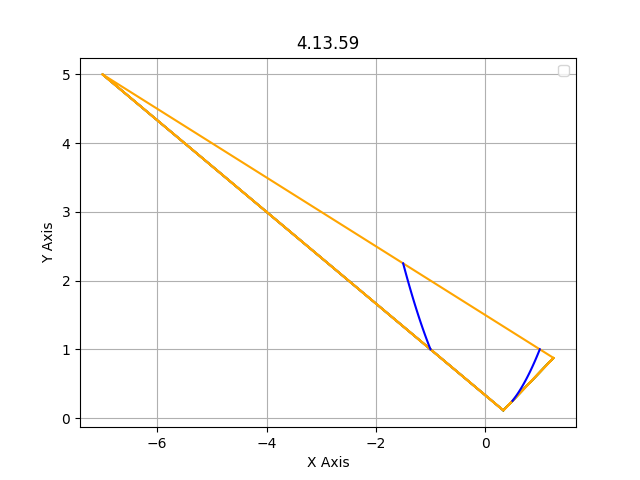
\includegraphics{figs/plot.png}
    \caption*{}
    \label{fig:plot}
\end{figure}
\end{document}
